85. $f(x)=\begin{cases} 2, \text{ если } x>1,\\ -1, \text{ если } x<1,\\ 1, \text{ если } x=1.\end{cases}$
Так как $\sqrt{x-2}=1$ при $x=3,\ f(\sqrt{x-2})=1$ при $x=3.$ Так как $\sqrt{x-2}>1$ при $x>3,\ f(\sqrt{x-2})=2$ при $x>3.$ При $x\in[2;3)$ имеем неравенство
$\sqrt{x-2}<1,$ значит $f(\sqrt{x-2})=-1$ при $x\in[2;3).$ Исходя их этого, построим график.
\begin{figure}[ht!]
\center{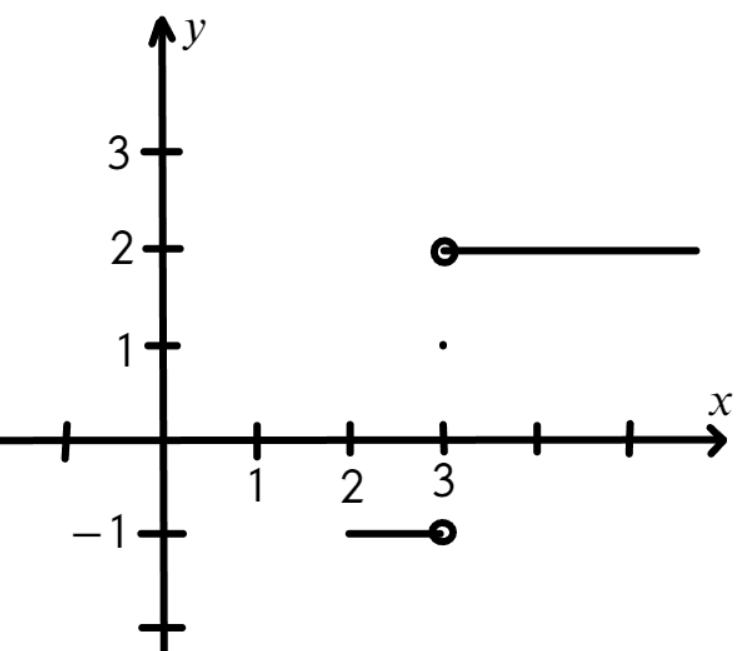
\includegraphics[scale=0.35]{gr9-85.png}}
\end{figure}\\
